\documentclass[12pt]{article}
\usepackage[utf8]{inputenc}
\usepackage{amsmath}
\usepackage{amsthm}
\usepackage{amsfonts}
\usepackage{amssymb}
\usepackage{mathtools}
\usepackage{pgfplots}
\usepackage{multirow}
\usepackage{pdfpages}
\usepackage{float}
\usepackage{listings}

\begin{document}

\def\arraystretch{1.2}%

Tobias Hille\hspace{1cm}
tobias.hille@student.uni-tuebingen.de\hspace{1cm}3905597\\
Robin Schmidt\hspace{1cm}
rob.schmidt@student.uni-tuebingen.de\hspace{1cm}4255055\\
\section*{Modellierung \& Simulation I}
%\subsection*{Serie 01}
\subsubsection*{1.1.1}
Empirische Wahrscheinlichkeit für einen Gewinn:
\begin{align*}
h(A) = \frac{n_i}{n} = \frac{283789}{2300000} \approx 0.12339
\end{align*}
Wahrscheinlichkeit unter der Laplace-Annahme:
\begin{align*}
p(A) = \frac{m_i}{m} = \frac{3^3}{6^3} = \frac{27}{216} = 0.125
\end{align*}
\subsubsection*{1.1.2}
Wertebereiche der Zufallsvariablen:
\begin{align*}
X_{sum} & \in \{ 2, 3, 4, 5, 6,7,8,9,10,11,12\} \\
X_{min} & \in \{1, 2, 3, 4, 5, 6\}\\
X_{max} & \in \{1, 2, 3, 4, 5, 6\}\\
X_{diff1} & \in \{0, 1, 2, 3, 4, 5\}\\
X_{diff2} & \in \{-5, -4, -3, -2, -1, 0, 1, 2, 3, 4, 5\}
\end{align*}
Verteilung und Verteilungsfunktionen der Zufallsvariablen:\\

\newpage
\begin{center}
\begin{tabular}{|c|c|c|c|c|c|c|c|c|c|c|c|}
\hline 
$x_i$ & 2 & 3 & 4 & 5 & 6 & 7 & 8 & 9 & 10 & 11 & 12 \\ 
\hline 
$P(X_{sum}=x_i)$ & $\frac{1}{36}$ & $\frac{2}{36}$ & $\frac{3}{36}$ & $\frac{4}{36}$ & $\frac{5}{36}$ & $\frac{6}{36}$ & $\frac{5}{36}$ & $\frac{4}{36}$ & $\frac{3}{36}$ & $\frac{2}{36}$ & $\frac{1}{36}$ \\ 
\hline 
$A(x_i)$ & $\frac{1}{36}$ & $\frac{3}{36}$ & $\frac{6}{36}$ & $\frac{10}{36}$ & $\frac{15}{36}$ & $\frac{21}{26}$ & $\frac{36}{36}$ & $\frac{30}{36}$ & $\frac{33}{36}$ & $\frac{35}{36}$ & $\frac{36}{36}$\\ 
\hline 
\end{tabular}
\vspace{0.5cm}\\

\begin{tikzpicture}
\begin{axis}[
ybar,
symbolic x coords={2,3,4,5,6,7,8,9,10,11,12},
ylabel={$P(X_{sum}=x_i)$},
xtick=data]
\addplot table [x=x, y=y, col sep=comma] {serie_01/data/x_sum.txt};
\end{axis}
\end{tikzpicture}

\begin{tikzpicture}
\begin{axis}[
symbolic x coords={2,3,4,5,6,7,8,9,10,11,12},
ylabel={$A(x_i)$},
xtick=data]
\addplot+ [jump mark left] table [x=x, y=y, col sep=comma] {serie_01/data/x_sum_a.txt};
\end{axis}
\end{tikzpicture}
\end{center}

\newpage
\begin{center}
\begin{tabular}{|c|c|c|c|c|c|c|}
\hline 
$x_i$ & 1 & 2 & 3 & 4 & 5 & 6 \\ 
\hline 
$P(X_{min}=x_i)$ & $\frac{11}{36}$ & $\frac{9}{36}$ & $\frac{7}{36}$ & $\frac{5}{36}$ & $\frac{3}{36}$ & $\frac{1}{36}$ \\ 
\hline 
$A(x_i)$ & $\frac{11}{36}$ & $\frac{20}{36}$ & $\frac{27}{36}$ & $\frac{32}{36}$ & $\frac{35}{36}$ & $\frac{36}{36}$ \\ 
\hline 
\end{tabular} 
\vspace{0.5cm}\\

\begin{tikzpicture}
\begin{axis}[
ybar,
symbolic x coords={1,2,3,4,5,6},
ylabel={$P(X_{min}=x_i)$},
xtick=data]
\addplot table [x=x, y=y, col sep=comma] {serie_01/data/x_min.txt};
\end{axis}
\end{tikzpicture}

\begin{tikzpicture}
\begin{axis}[
symbolic x coords={1,2,3,4,5,6},
ylabel={$A(x_i)$},
xtick=data]
\addplot+ [jump mark left] table [x=x, y=y, col sep=comma] {serie_01/data/x_min_a.txt};
\end{axis}
\end{tikzpicture}
\end{center}

\newpage
\begin{center}
\begin{tabular}{|c|c|c|c|c|c|c|}
\hline 
$x_i$ & 1 & 2 & 3 & 4 & 5 & 6 \\ 
\hline 
$P(X_{max}=x_i)$ & $\frac{1}{36}$ & $\frac{3}{36}$ & $\frac{5}{36}$ & $\frac{7}{36}$ & $\frac{9}{36}$ & $\frac{11}{36}$ \\ 
\hline 
$A(x_i)$ & $\frac{1}{36}$ & $\frac{4}{36}$ & $\frac{9}{36}$ & $\frac{16}{36}$ & $\frac{25}{36}$ & $\frac{36}{36}$ \\ 
\hline 
\end{tabular} 
\vspace{0.5cm}\\

\begin{tikzpicture}
\begin{axis}[
ybar,
symbolic x coords={1,2,3,4,5,6},
ylabel={$P(X_{max}=x_i)$},
xtick=data]
\addplot table [x=x, y=y, col sep=comma] {serie_01/data/x_max.txt};
\end{axis}
\end{tikzpicture}

\begin{tikzpicture}
\begin{axis}[
symbolic x coords={1,2,3,4,5,6},
ylabel={$A(x_i)$},
xtick=data]
\addplot+ [jump mark left] table [x=x, y=y, col sep=comma] {serie_01/data/x_max_a.txt};
\end{axis}
\end{tikzpicture}
\end{center}

\newpage
\begin{center}
\begin{tabular}{|c|c|c|c|c|c|c|}
\hline 
$x_i$ & 0 & 1 & 2 & 3 & 4 & 5 \\ 
\hline 
$P(X_{diff1}=x_i)$ & $\frac{6}{36}$ & $\frac{10}{36}$ & $\frac{8}{36}$ & $\frac{6}{36}$ & $\frac{4}{36}$ & $\frac{2}{36}$ \\ 
\hline 
$A(x_i)$ & $\frac{6}{36}$ & $\frac{16}{36}$ & $\frac{24}{36}$ & $\frac{30}{36}$ & $\frac{34}{36}$ & $\frac{36}{36}$ \\ 
\hline 
\end{tabular} 
\vspace{0.5cm}\\

\begin{tikzpicture}
\begin{axis}[
ybar,
symbolic x coords={0,1,2,3,4,5},
ylabel={$P(X_{diff1}=x_i)$},
xtick=data]
\addplot table [x=x, y=y, col sep=comma] {serie_01/data/x_diff1.txt};
\end{axis}
\end{tikzpicture}

\begin{tikzpicture}
\begin{axis}[
symbolic x coords={0,1,2,3,4,5},
ylabel={$A(x_i)$},
xtick=data]
\addplot+ [jump mark left] table [x=x, y=y, col sep=comma] {serie_01/data/x_diff1_a.txt};
\end{axis}
\end{tikzpicture}
\end{center}

\newpage
\begin{center}
\begin{tabular}{|c|c|c|c|c|c|c|c|c|c|c|c|}
\hline 
$x_i$ & -5 & -4 & -3 & -2 & -1 & 0 & 1 & 2 & 3 & 4 & 5 \\ 
\hline 
$P(X_{diff2}=x_i)$ & $\frac{1}{36}$ & $\frac{2}{36}$ & $\frac{3}{36}$ & $\frac{4}{36}$ & $\frac{5}{36}$ & $\frac{6}{36}$ & $\frac{5}{36}$ & $\frac{4}{36}$ & $\frac{3}{36}$ & $\frac{2}{36}$ & $\frac{1}{36}$ \\ 
\hline 
$A(x_i)$ & $\frac{1}{36}$ & $\frac{3}{36}$ & $\frac{6}{36}$ & $\frac{10}{36}$ & $\frac{15}{36}$ & $\frac{21}{26}$ & $\frac{26}{36}$ & $\frac{30}{36}$ & $\frac{33}{36}$ & $\frac{35}{36}$ & $\frac{36}{36}$\\ 
\hline 
\end{tabular}
\vspace{0.5cm}\\

\begin{tikzpicture}
\begin{axis}[
ybar,
symbolic x coords={-5,-4,-3,-2,-1,0,1,2,3,4,5},
ylabel={$P(X_{diff2}=x_i)$},
xtick=data]
\addplot table [x=x, y=y, col sep=comma] {serie_01/data/x_diff2.txt};
\end{axis}
\end{tikzpicture}

\begin{tikzpicture}
\begin{axis}[
symbolic x coords={-5,-4,-3,-2,-1,0,1,2,3,4,5},
ylabel={$A(x_i)$},
xtick=data]
\addplot+ [jump mark left] table [x=x, y=y, col sep=comma] {serie_01/data/x_diff2_a.txt};
\end{axis}
\end{tikzpicture}  
\end{center}

\newpage
Kenngrößen der Zufallsvariablen:

\begin{center}
\begin{tabular}{|c|c|c|}
\hline 
Zufallsgröße & Erwartungswert & Varianz \\ 
\hline 
$X_{sum}$ & 7 & 5.833333333333333 \\ 
\hline 
$X_{min}$ & 2.5277777777777777 & 1.9714506172839503
 \\ 
\hline 
$X_{max}$ & 4.472222222222222 & 1.9714506172839508
 \\ 
\hline 
$X_{diff1}$ & 1.9444444444444446 & 2.052469135802469 \\ 
\hline 
$X_{diff2}$ & 0 & 5.833333333333334 \\ 
\hline 
\end{tabular} 
\end{center}

\subsubsection*{1.1.3}
Wertebereich der Zufallsvariable:
\begin{align*}
X \in \{i | i\in\mathbb{N}, 1 \leq i < \infty \}
\end{align*}
Diese Zufallsvariabe folgt der geometrischen Verteilung. Die Verteilungsfunktion ist
\begin{align*}
x(i) = (1-p)^{i-1} \cdot p
\end{align*}
mit $p=\frac{1}{6}$.
Für die Wahrscheinlichkeit, höchstens vier Würfe bis zum ersten Auftreten der Augenzahl 6, ergibt sich:
\begin{align*}
P(i \leq 4 ) = \sum_{k=1}^4 \frac{5}{6}^{k-1} \cdot \frac{1}{6} = 0.5177
\end{align*}
\subsubsection*{1.2.1}
Geometrische Verteilung $P_{geo}(X=n)=p (1-p)^{n}$ mit $p = 0.5$ :

\begin{center}
\begin{tikzpicture}
\begin{axis}[
ybar,
symbolic x coords={0,1,2,3,4,5,6,7,8,9,10},
ylabel={$P_{geo}(X)$},
xtick=data]
\addplot table [x=x, y=y, col sep=comma] {serie_01/data/geom.txt};
\end{axis}
\end{tikzpicture}
\end{center}
\vspace{0.5cm}
Exponentielle Verteilung $f_{\lambda}(x) = \begin{cases} \lambda e^{-\lambda x} & x \geq 0 \\ 0 & x < 0\end{cases}$ mit $\lambda = 2$ (grün), $\lambda = 1$ (blau) und $\lambda = 0.75$ (rot):
\begin{center}
\vspace{0.5cm}
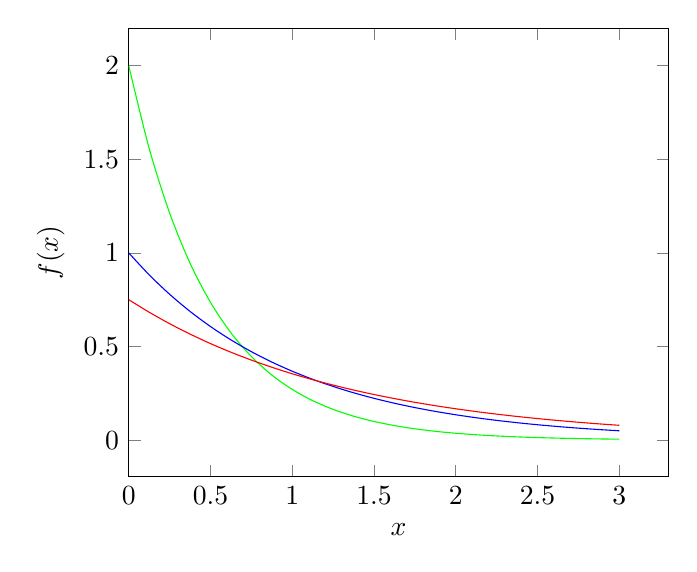
\begin{tikzpicture}
  \begin{axis}[ 
    xlabel=$x$,
    xmin=0,
    smooth,
    domain=0:3,
    ylabel={$f(x)$}
  ] 
    \addplot [color=green] {2*exp(-2*x)};
    \addplot [color=blue] {1*exp(-1*x)};
    \addplot [color=red] {0.75*exp(-0.75*x)};
  \end{axis}
\end{tikzpicture}
\end{center}
\subsubsection*{1.2.2}
Verteilungsdichtefunktion der geometrischen Verteilung für $p = 0.5$:
\begin{center}
\begin{tikzpicture}
\begin{axis}[
symbolic x coords={0,1,2,3,4,5,6,7,8,9,10},
ylabel={$P_{geo}(X)$},
xtick=data]
\addplot+ [jump mark left] table [x=x, y=y, col sep=comma] {serie_01/data/geom_a.txt};
\end{axis}
\end{tikzpicture}
\end{center}
Verteilungsdichtefunktion $F_\lambda$ der exponentiellen Verteilung mit $\lambda = 2$ (grün), $\lambda = 1$ (blau) und $\lambda = 0.75$ (rot):
\begin{equation*}
    F_{\lambda}(x) = \int_0^x \! f_\lambda(x) \, \mathrm{d}x = \begin{cases} 1 - e^{-\lambda x} & x \geq 0 \\ 0 & x < 0\end{cases} 
\end{equation*}

\vspace{0.5cm}
\begin{center}
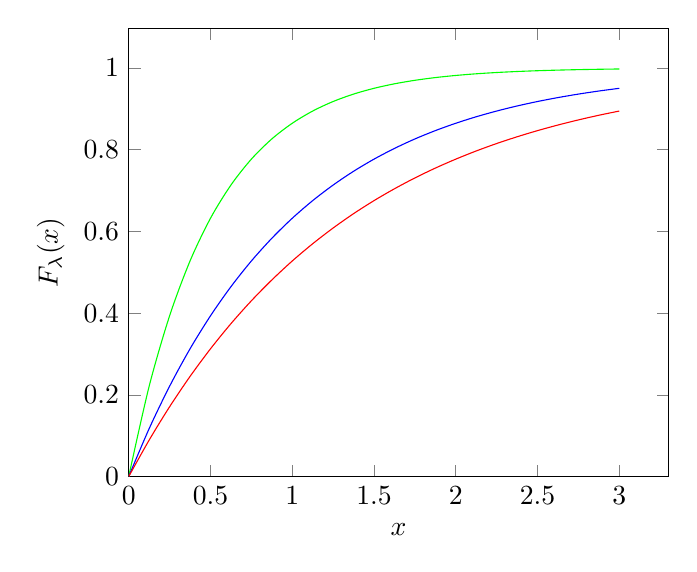
\begin{tikzpicture}
  \begin{axis}[ 
    xlabel=$x$,
    xmin=0,
    ymin=0,
    smooth,
    domain=0:3,
    ylabel={$F_\lambda(x)$}
  ] 
    \addplot [color=green] {1-(exp(-2*x))};
    \addplot [color=blue] {1-(exp(-1*x))};
    \addplot [color=red] {1-(exp(-0.75*x))};
  \end{axis}
\end{tikzpicture}
\end{center}
Unterschied: Die geometrische Verteilung ist diskret und die exponentielle Verteilung ist kontinuierlich. Dies liegt daran, dass die exponentielle Verteilung als Grenzfall aus der geometrischen Verteilung für $X$ herausgeht, wenn $p=1/n$ und $\frac{X}{n}$ für $n\xrightarrow{}\infty$ betrachtet wird.

\subsubsection*{1.2.3}
Wahrscheinlichkeit für $P(X\leq1)$ für die geometrische und exponentielle Verteilung:
\begin{align*}
P_{geo}(X \leq 1) & = 1-(1-p)^1 = p\\
P_{exp}(X \leq 1) & = 1-e^{-\lambda\cdot1} = 1-e^{-\lambda}
\end{align*}
\subsection*{Serie 02}
\subsubsection*{Problem 2.2.1}
The discrete event simulation (DES) has various components, which work together to successfully simulate discrete events. These components include the simulation clock, events, statistic counters and the main program. 

The simulation clock shows the current system time. Here the real time needs to be converted to the corresponding simulation time. Events are associated with a discrete simulation time, at which the event runs his corresponding event routine. An event routine leads to an action in the system which can influence for example the system state. All events are managed in an event chain (event queue). Statistic counters contain information about the system, which can be for example packet sizes or queue lengths. 

The first step in the main program is to initialize the system state, containing variables, lists and queues. After everything is initialized the event chain gets executed. During this process the next event in the event chain gets selected, the simulation time gets forwarded to the event time and finally the event routine gets executed. While the event chain is being executed, the size of the chain is always greater than $1$ because of the terminating stop event. Once the termination event is reached, the simulation process terminates. 
\newpage
\subsubsection*{Problem 2.2.4}
Results of simulation $1$ with an interarrival time of customers $10s$, service time $9s$ and simulation time $10000s$:
\begin{table}[h]
\centering
\begin{tabular}{|l|l|l|}
\hline
\multirow{2}{*}{} & \multicolumn{2}{l|}{Simulation 1} \\ \cline{2-3} 
                  & $mean$        & $c_{var}$      \\ \hline
occupancy time    & 0.0           & 0.0             \\ \hline
service time      & 9.0           & 0.0             \\ \hline
utilization time  & 0.9           & 0.33333333333333326              \\ \hline
waiting time & 0.0         & 0.0             \\ \hline
\end{tabular}
\end{table}\\
Results of simulation $2$ with an interarrival time of customers $10s$, service time $10s$ and simulation time $10000s$:
\begin{table}[h]
\centering
\begin{tabular}{|l|l|l|}
\hline
\multirow{2}{*}{} & \multicolumn{2}{l|}{Simulation 2} \\ \cline{2-3} 
                  & $mean$        & $c_{var}$      \\ \hline
occupancy time      & 0.0           & 0.0            \\ \hline
service time      & 10.0           & 0.0            \\ \hline
utilization time  & 1.0           & 0.0             \\ \hline
waiting time & 0.0         & 0.0             \\ \hline
\end{tabular}
\end{table}\\
Results of simulation $3$ with an interarrival time of customers $10s$, service time $11s$ and simulation time $10000s$:
\begin{table}[h]
\centering
\begin{tabular}{|l|l|l|}
\hline
\multirow{2}{*}{} & \multicolumn{2}{l|}{Simulation 3} \\ \cline{2-3} 
                  & $mean$        & $c_{var}$      \\ \hline
occupancy time      & 44.865           & 0.5849120747543387            \\ \hline
service time      & 11.0           & 0.0            \\ \hline
utilization time  & 1.0           & 0.0             \\ \hline
waiting time & 454.0         & 0.5783039542709295             \\ \hline
\end{tabular}
\end{table}\\
\newpage
\noindent Results of simulation $4$ with an interarrival time of customers $10s$, service time $9s$ and simulation time $100000s$:
\begin{table}[h]
\centering
\begin{tabular}{|l|l|l|}
\hline
\multirow{2}{*}{} & \multicolumn{2}{l|}{Simulation 4} \\ \cline{2-3} 
                  & $mean$        & $c_{var}$      \\ \hline
occupancy time      & 0.0           & 0.0            \\ \hline
service time      & 9.0           & 0.0            \\ \hline
utilization time  & 0.9           & 0.33333333333333326             \\ \hline
waiting time & 0.0         & 0.0             \\ \hline
\end{tabular}
\end{table}\\
Results of simulation $5$ with an interarrival time of customers $10s$, service time $10s$ and simulation time $100000s$:
\begin{table}[h]
\centering
\begin{tabular}{|l|l|l|}
\hline
\multirow{2}{*}{} & \multicolumn{2}{l|}{Simulation 5} \\ \cline{2-3} 
                  & $mean$        & $c_{var}$      \\ \hline
occupancy time      & 0.0           & 0.0            \\ \hline
service time      & 10.0           & 0.0            \\ \hline
utilization time  & 1.0           & 0.0             \\ \hline
waiting time & 0.0         & 0.0             \\ \hline
\end{tabular}
\end{table}\\
Results of simulation $6$ with an interarrival time of customers $10s$, service time $11s$ and simulation time $100000s$:
\begin{table}[h]
\centering
\begin{tabular}{|l|l|l|}
\hline
\multirow{2}{*}{} & \multicolumn{2}{l|}{Simulation 6} \\ \cline{2-3} 
                  & $mean$        & $c_{var}$      \\ \hline
occupancy time      & 453.9546           & 0.5781011743810226            \\ \hline
service time      & 11.0           & 0.0            \\ \hline
utilization time  & 1.0           & 0.0             \\ \hline
waiting time & 4544.5         & 0.5774455511199658             \\ \hline
\end{tabular}
\end{table}
\newpage
\subsubsection*{Problem 2.2.5}
Histogram for waiting and service time per customer for simulation $1$:\\
\begin{figure}[H]
	\centering
  \includegraphics[width=0.7\textwidth]{serie_02/data/Simulation1/waiting_time.pdf}
	\caption{Simulation 1 - Waiting Time}
	\label{fig3}
\end{figure}
\begin{figure}[H]
	\centering
  \includegraphics[width=0.7\textwidth]{serie_02/data/Simulation1/service_time.pdf}
	\caption{Simulation 1 - Service Time}
	\label{fig3}
\end{figure}
\newpage
Histogram for waiting and service time per customer for simulation $2$:\\
\begin{figure}[H]
	\centering
  \includegraphics[width=0.7\textwidth]{serie_02/data/Simulation2/waiting_time.pdf}
	\caption{Simulation 2 - Waiting Time}
	\label{fig3}
\end{figure}

\begin{figure}[H]
	\centering
  \includegraphics[width=0.7\textwidth]{serie_02/data/Simulation2/service_time.pdf}
	\caption{Simulation 2 - Service Time}
	\label{fig3}
\end{figure}
\newpage
Histogram for waiting and service time per customer for simulation $3$:\\

\begin{figure}[H]
	\centering
  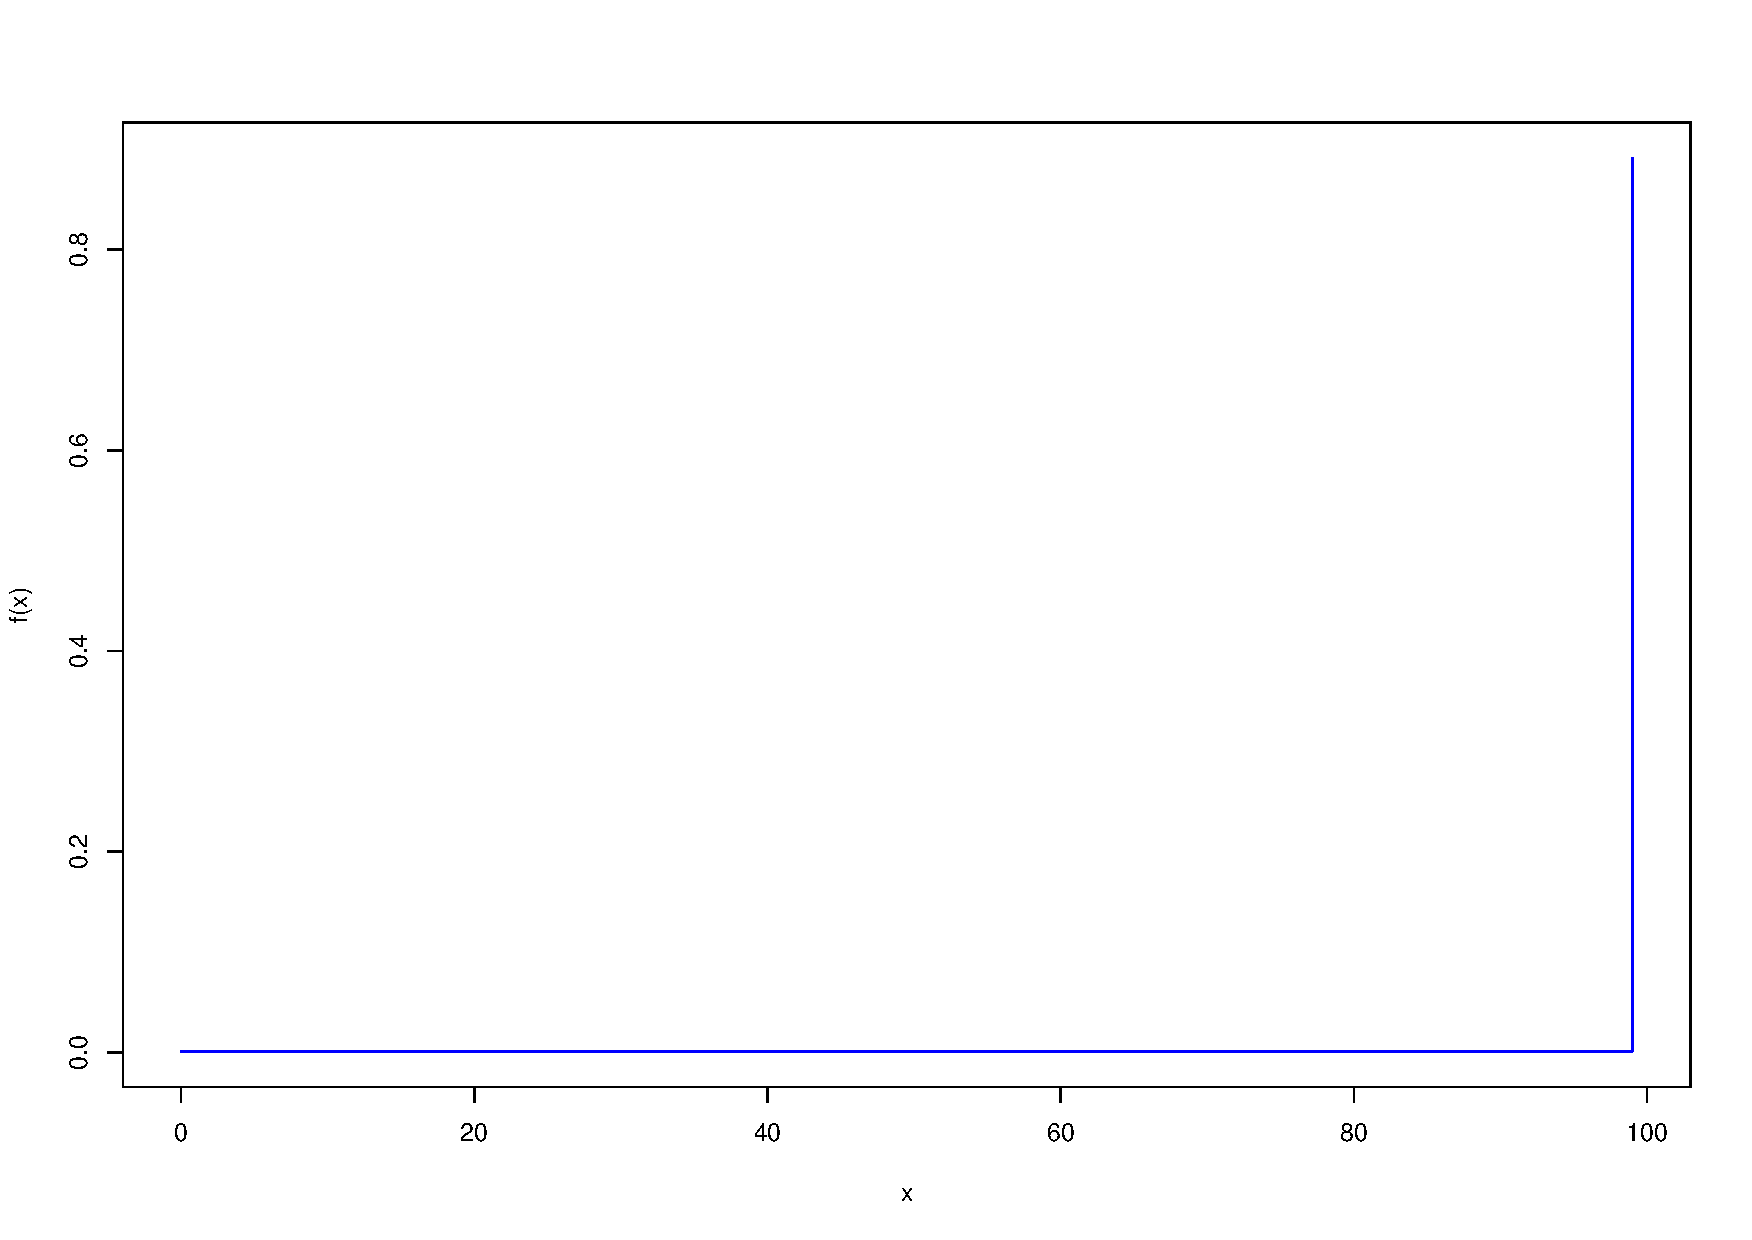
\includegraphics[width=0.7\textwidth]{serie_02/data/Simulation3/waiting_time.pdf}
	\caption{Simulation 3 - Waiting Time}
	\label{fig3}
\end{figure}

\begin{figure}[H]
	\centering
  \includegraphics[width=0.7\textwidth]{serie_02/data/Simulation3/service_time.pdf}
	\caption{Simulation 3 - Service Time}
	\label{fig3}
\end{figure}
\newpage
Histogram for waiting and service time per customer for simulation $4$:\\

\begin{figure}[H]
	\centering
  \includegraphics[width=0.7\textwidth]{serie_02/data/Simulation4/waiting_time.pdf}
	\caption{Simulation 4 - Waiting Time}
	\label{fig3}
\end{figure}

\begin{figure}[H]
	\centering
  \includegraphics[width=0.7\textwidth]{serie_02/data/Simulation4/service_time.pdf}
	\caption{Simulation 4 - Service Time}
	\label{fig3}
\end{figure}
\newpage
Histogram for waiting and service time per customer for simulation $5$:\\

\begin{figure}[H]
	\centering
  \includegraphics[width=0.7\textwidth]{serie_02/data/Simulation5/waiting_time.pdf}
	\caption{Simulation 5 - Waiting Time}
	\label{fig3}
\end{figure}

\begin{figure}[H]
	\centering
  \includegraphics[width=0.7\textwidth]{serie_02/data/Simulation5/service_time.pdf}
	\caption{Simulation 5 - Service Time}
	\label{fig3}
\end{figure}
\newpage
Histogram for waiting and service time per customer for simulation $6$:\\

\begin{figure}[H]
	\centering
  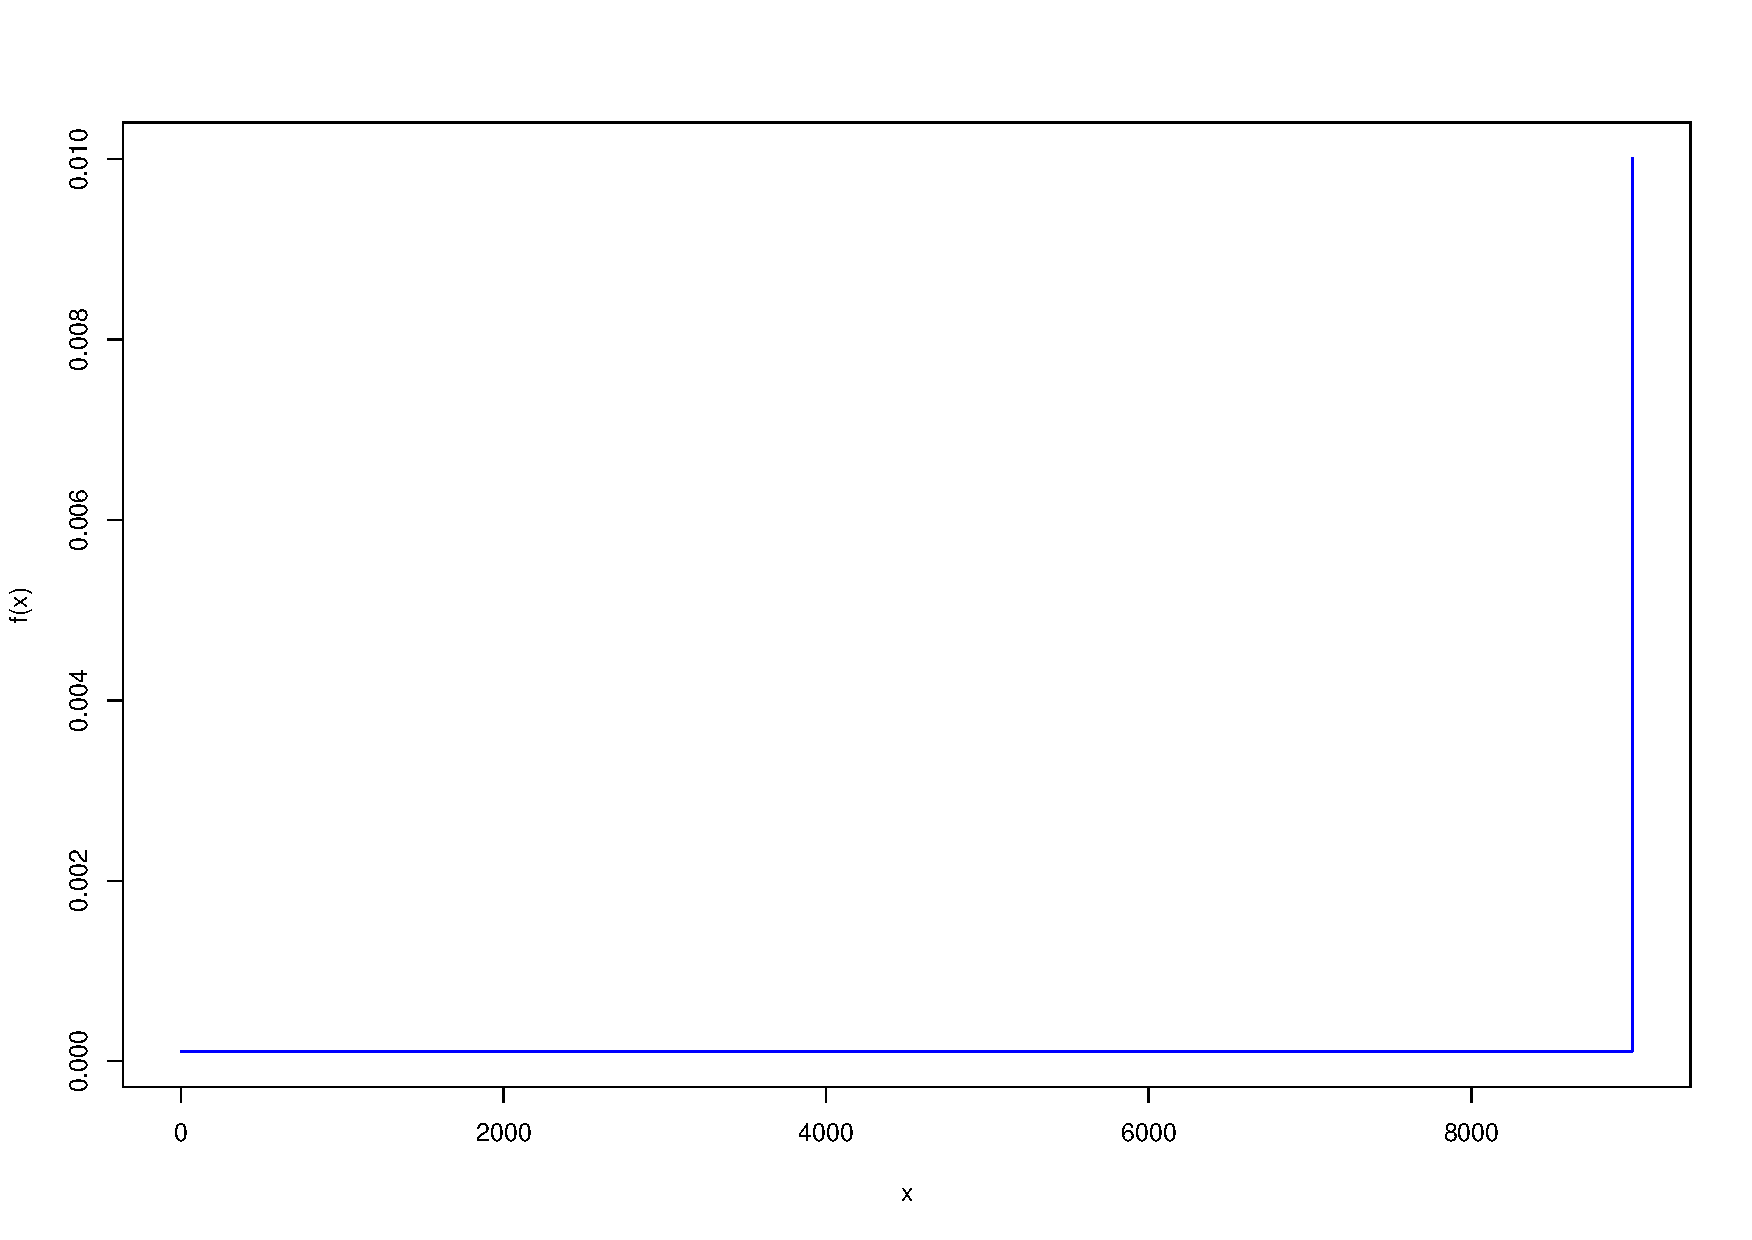
\includegraphics[width=0.7\textwidth]{serie_02/data/Simulation6/waiting_time.pdf}
	\caption{Simulation 6 - Waiting Time}
	\label{fig3}
\end{figure}

\begin{figure}[H]
	\centering
  \includegraphics[width=0.7\textwidth]{serie_02/data/Simulation6/service_time.pdf}
	\caption{Simulation 6 - Service Time}
	\label{fig3}
\end{figure}

\subsubsection*{Problem 2.2.6}
Discrete counter instead of continous counter for queue occupancy and server utilization:\\
Comparison of mean values and the coefficient of the variation with above: 




\subsubsection*{Problem 2.3.1}
\textit{please see code}
\subsubsection*{Problem 2.3.2}
\textit{please see code}
\subsubsection*{Problem 2.3.3}

The Exponential distributions with $mean=1$, $c_{var} = 0.1$ and $mean=1$, $c_{var}=2$ cannot be instantiated. This is because the relation $c_{var}=\frac{\sigma}{mean}=\frac{\sqrt{\frac{1}{\lambda^2}}}{\frac{1}{\lambda}}= 1$ is not fulfilled.\\
The ErlangK distribution with $mean=1$,$c_{var}=2$ cannot be instantiated. This is because the relation
$c_{var} = \frac{\sigma}{mean} = \frac{\frac{\sqrt{k}}{\lambda}}{\frac{k}{\lambda}} = \frac{1}{\sqrt{k}}$ is not true for any integer k.\\
The HyperExponential distribution H2 with $mean=1$, $c_{var} = 0.1$ cannot be instantiated. This is because $c_{var}^2 - 1$ has to be greater or equal $0$.\\
The HyperExponential distribution H2 with $mean=1$, $c_{var}=1$ can be instantiated, but because the two resulting lambda's are the same, the two probabilities p are the same too. It follows, that this is a degenerated hyperexponential distribution and behaves just like a "normal" exponential distribution.

The following pages contain the console output for a specific run of the RandVarTest.java file.\\
\lstinputlisting[language={}]{./serie_02/var_test_console.txt}

\end{document}